\documentclass[11pt, answers]{exam}
\usepackage[margin=1in]{geometry}
\usepackage{amsfonts, amsmath, amssymb, amsthm}
\usepackage{mathtools}
\usepackage{enumerate}
\usepackage{listings}
\usepackage{hyperref}
\usepackage[boxed]{algorithm}
\usepackage[noend]{algpseudocode}
\usepackage{tikz}
\usepackage{multirow}
\usepackage{float}

%
% Basic Document Settings
%

\topmargin=-0.45in
\evensidemargin=0in
\oddsidemargin=0in
\textwidth=6.5in
\textheight=9.0in
\headsep=0.25in

\linespread{1.1}

\pagestyle{headandfoot}
\lhead{\hmwkAuthorName\ (\hmwkUniqname)}
\rhead{\hmwkClass\ : \hmwkType\ \#\hmwkNumber\ (Due \hmwkDue)}
\cfoot{\thepage}
% \renewcommand\headrulewidth{0.4pt}
% \renewcommand\footrulewidth{0.4pt}

\setlength\parindent{0pt}

%
% Create Problem Sections
%
\qformat{\hfill}

\newcommand{\hmwkType}{Project}
\newcommand{\hmwkNumber}{2}
\newcommand{\hmwkClass}{EECS 445}
\newcommand{\hmwkDue}{Tuesday, March 31th at 11:59pm}
\newcommand{\hmwkAuthorName}{\textbf{Yihao Huang}}
\newcommand{\hmwkUniqname}{\textbf{yihaoh}}


%
% Title Page
%

\author{\hmwkAuthorName}

%
% Various Helper Commands
%

% space of real numbers \R
\newcommand{\R}{\mathbb{R}}

% expected value \EX
\DeclareMathOperator{\EX}{\mathbb{E}}

% For partial derivatives \pderiv{}{}
\newcommand{\pderiv}[2]{\frac{\partial}{\partial #1} (#2)}

% argmax \argmax
\DeclareMathOperator*{\argmax}{arg\,max}

% sign \sign
\DeclareMathOperator{\sign}{sign}

% norm \norm{}
\DeclarePairedDelimiter{\norm}{\lVert}{\rVert}

% Keys
\newcommand{\key}[1]{\fbox{{\sc #1}}}
\newcommand{\ctrl}{\key{ctrl}--}
\newcommand{\shift}{\key{shift}--}
\newcommand{\run}{\key{run} \ }
\newcommand{\runkey}[1]{\run \key{#1}}
\newcommand{\extend}{\key{extend} \ }
\newcommand{\kkey}[1]{\key{k$_{#1}$}}

\begin{document}
  \section{Data Preprocessing}%
  \label{sec:introduction}

  \begin{solution}\begin{parts}
    \part
    \part The resulting mean and standard deviation are shown in the table below\\
    \begin{center}
      \begin{tabular}{c|ccc}
       & R& G& B\\
      \hline
      mean& 139.227 & 114.107 & 88.359\\
      standard deviation& 65.071 & 65.904 & 67.451\\
      \end{tabular}
    \end{center}
    
    We extract the per-channel image mean and standard deviation from the training set because by doing so, the potential of the model being overfitting is reduced. If we extract the per-channel image mean and standard deviation from both the training set and the testing set, then information of testing set will be included and thus the model has the potential to be overfitting.

    \part ~\\
    \begin{center}
      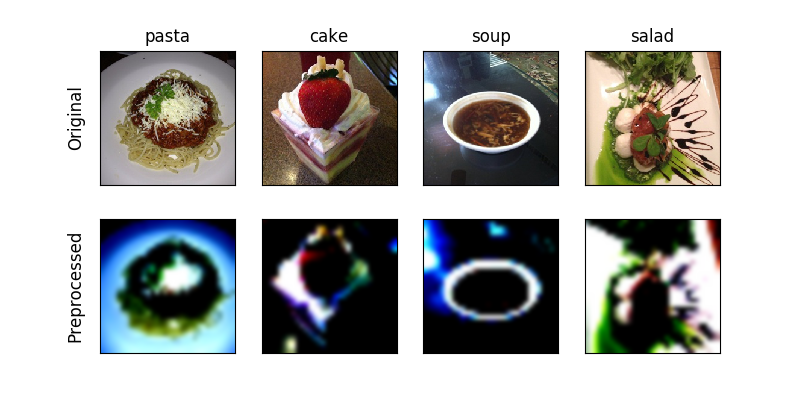
\includegraphics[scale=0.7]{Figure_1.png}
    \end{center}

    After preprocessing, images become blurred and detailed information are lost, as we have resized them into a smaller size. For example, at the top of the image of salad, after preprocessing, it is hard to see that there are actually bunch of vegetable leaves there. Besides, the dark parts becomes darker and the bright parts become brighter, as the results of the standardizing process.
  \end{parts}\end{solution}

  \section{Convolutional Neural Networks}%
  \label{sec:convolutional_neural_networks}

  \begin{solution}
  \begin{parts}
    \part
      \begin{center}
        \begin{tabular}{c|ccc}
          layer& weight& bias& total parameters\\
          \hline
          0 & 0 & 0 & 0\\
          1 & $3\times 5\times 5\times 16$ & 16 & 1216\\
          2 & $16\times 5\times 5\times 64$ & 64 & 25664\\
          3 & $64\times 5\times 5\times 32$ & 32 & 51232\\
          4 & $512\times 64$ & 64 & 32832\\
          5 & $64\times 32$ & 32 & 2080\\
          6 & $32\times 5$ & 5 & 165
        \end{tabular}
    \end{center}

    Therefore, in all, there are $1216 + 25664 + 51232 + 32832 + 2080 + 165 = 113189$ learnable float-valued parameters.

    \part
    \part
    \part
    \part The training results are shown in the figure below.
    \begin{center}
      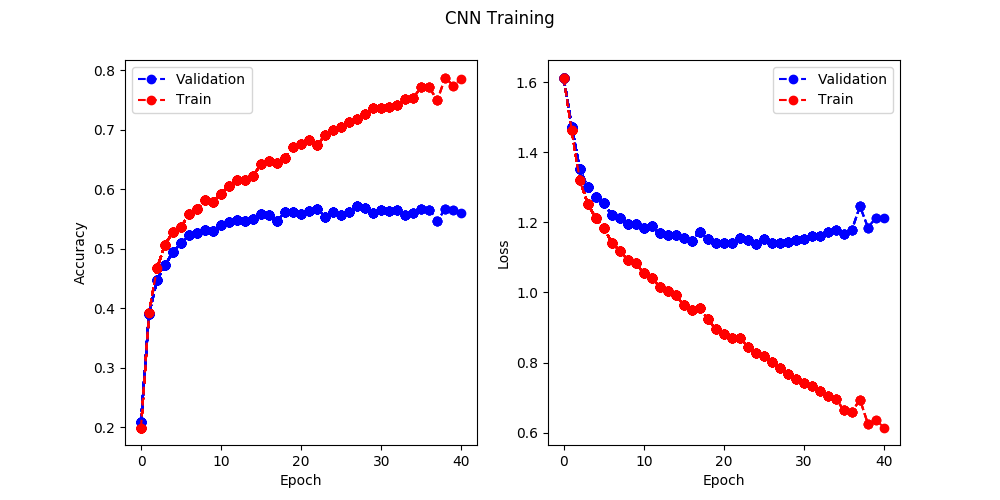
\includegraphics[scale=0.6]{eecs445-p2-2e.png}
    \end{center}

    \begin{enumerate}[i.]
      \item The first source of noise might be the preprocessing we have used. As we have resized and standardize the graphes, there might be information loss, which lead to the fluctuation of the training loss. The second source of noise is due to the SGD training process we are using. As a feature of SGD, the validation loss would not monotonically decrease at the beginning, because the update is made based on a single data point. 

      \item If we were to continue training the model, the training loss will continue to decrease monotonically until it reaches some certain value,  while the validation loss will increase. It can be seen in the graph that the validation loss start to increase after about epoch 25. Combined with the fact that the training loss continues to decrease, the conclusion can be drawn that the model starts to overfit.

      \item The training should be stopped at epoch 27, because after this point, the validation loss starts to increase, indicating that the model starts to overfit, and the validation accuracy of this epoch is the highest among those epoch having close validation loss.
    \end{enumerate}

    \part ~\\
    \begin{center}
      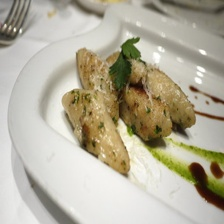
\includegraphics[scale=0.3]{00015.jpg}
      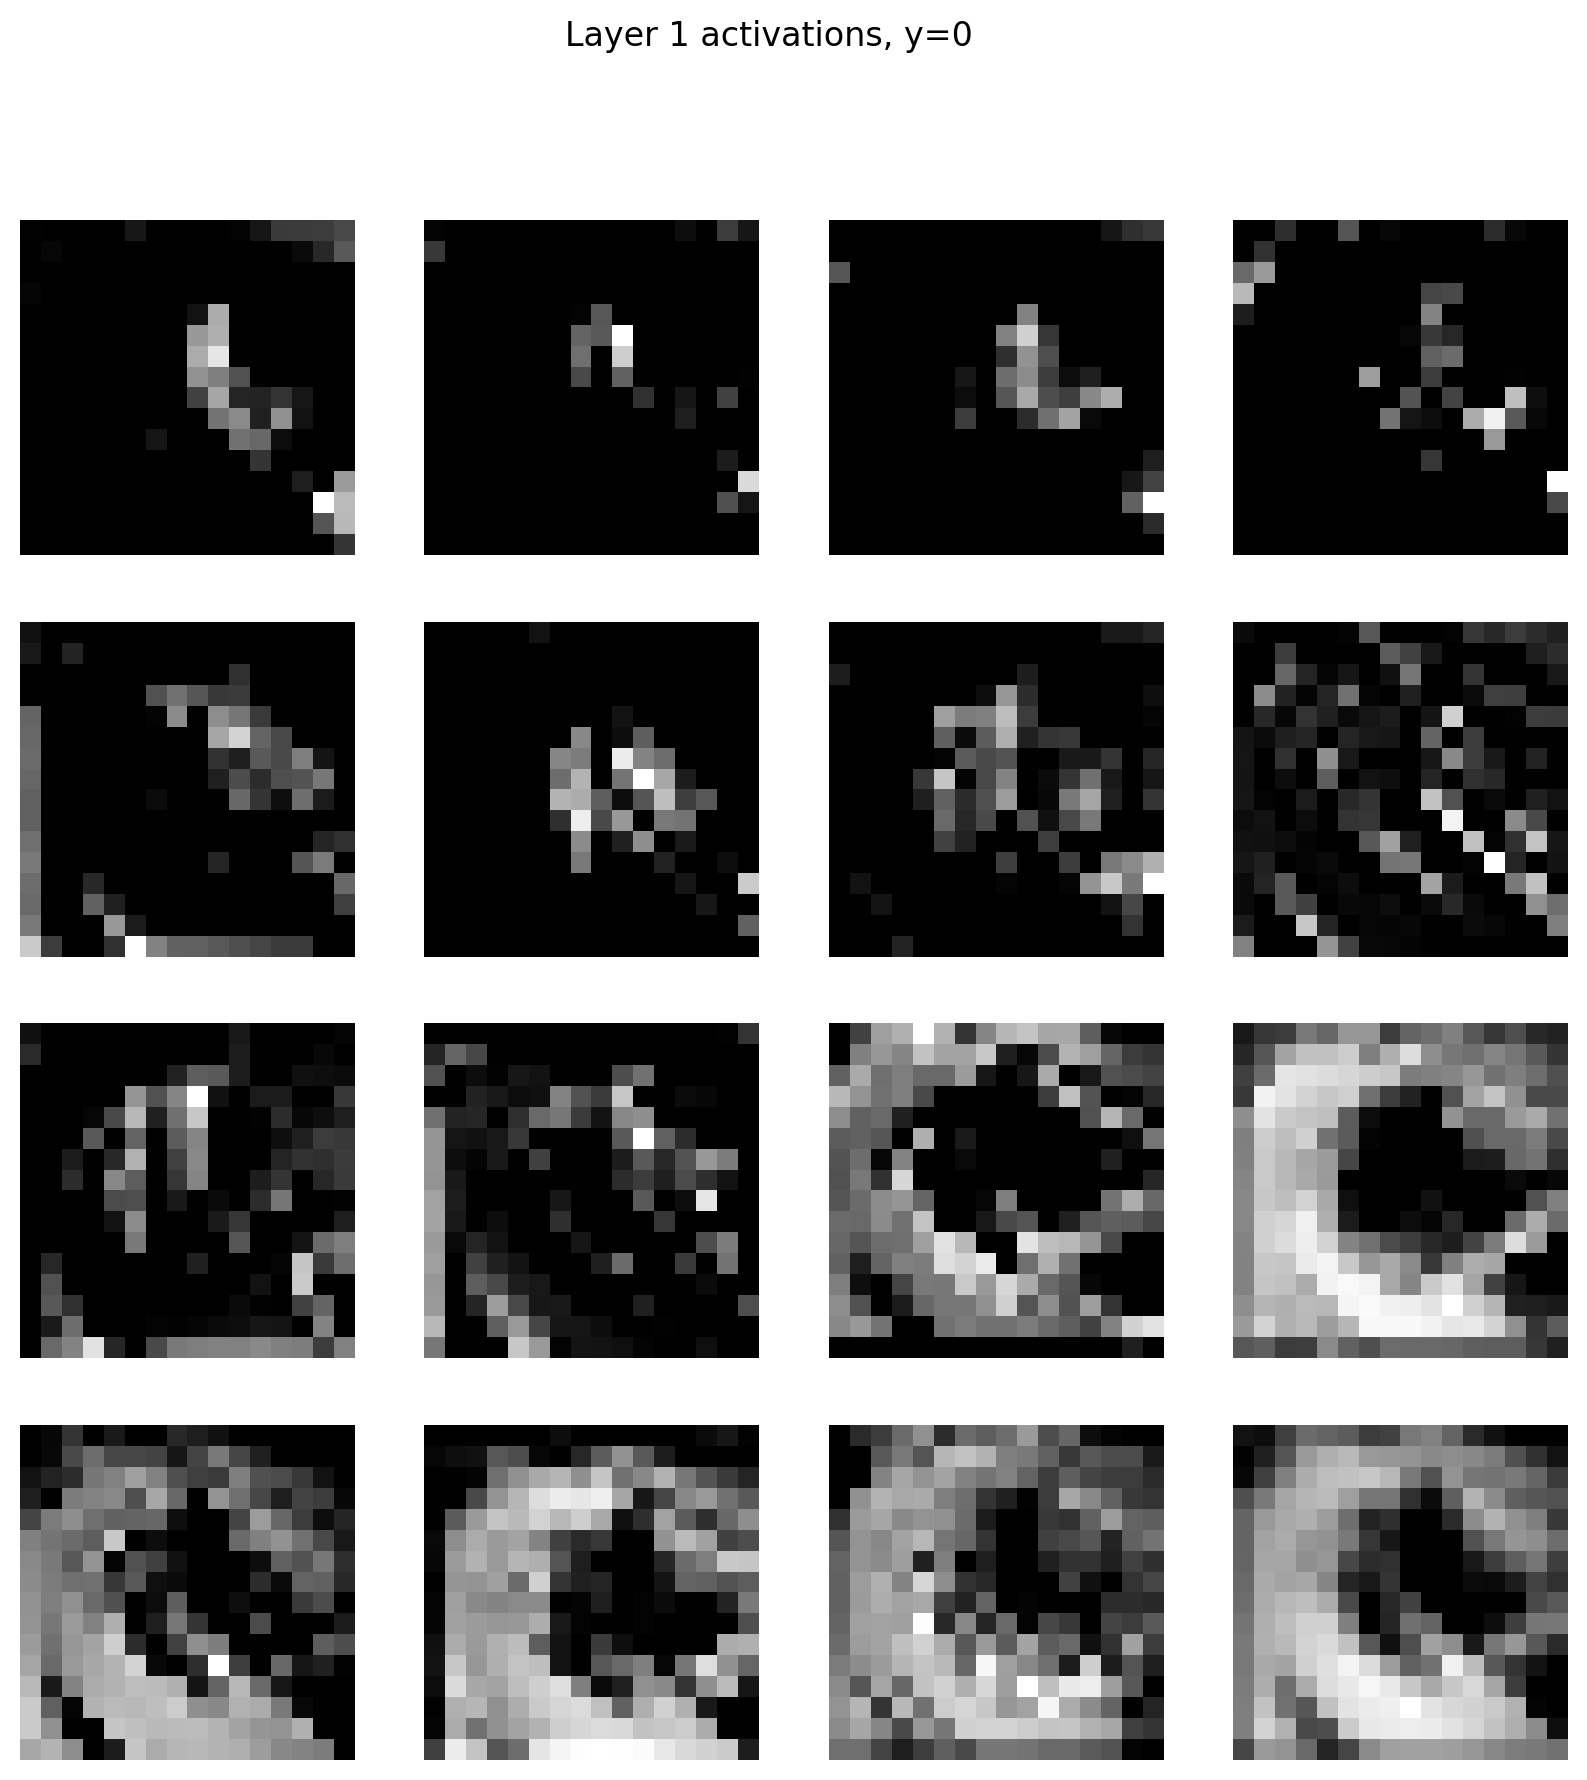
\includegraphics[scale=0.6]{CNN_viz1_0.png}
      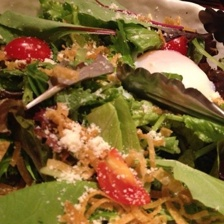
\includegraphics[scale=0.3]{00021.jpg}
      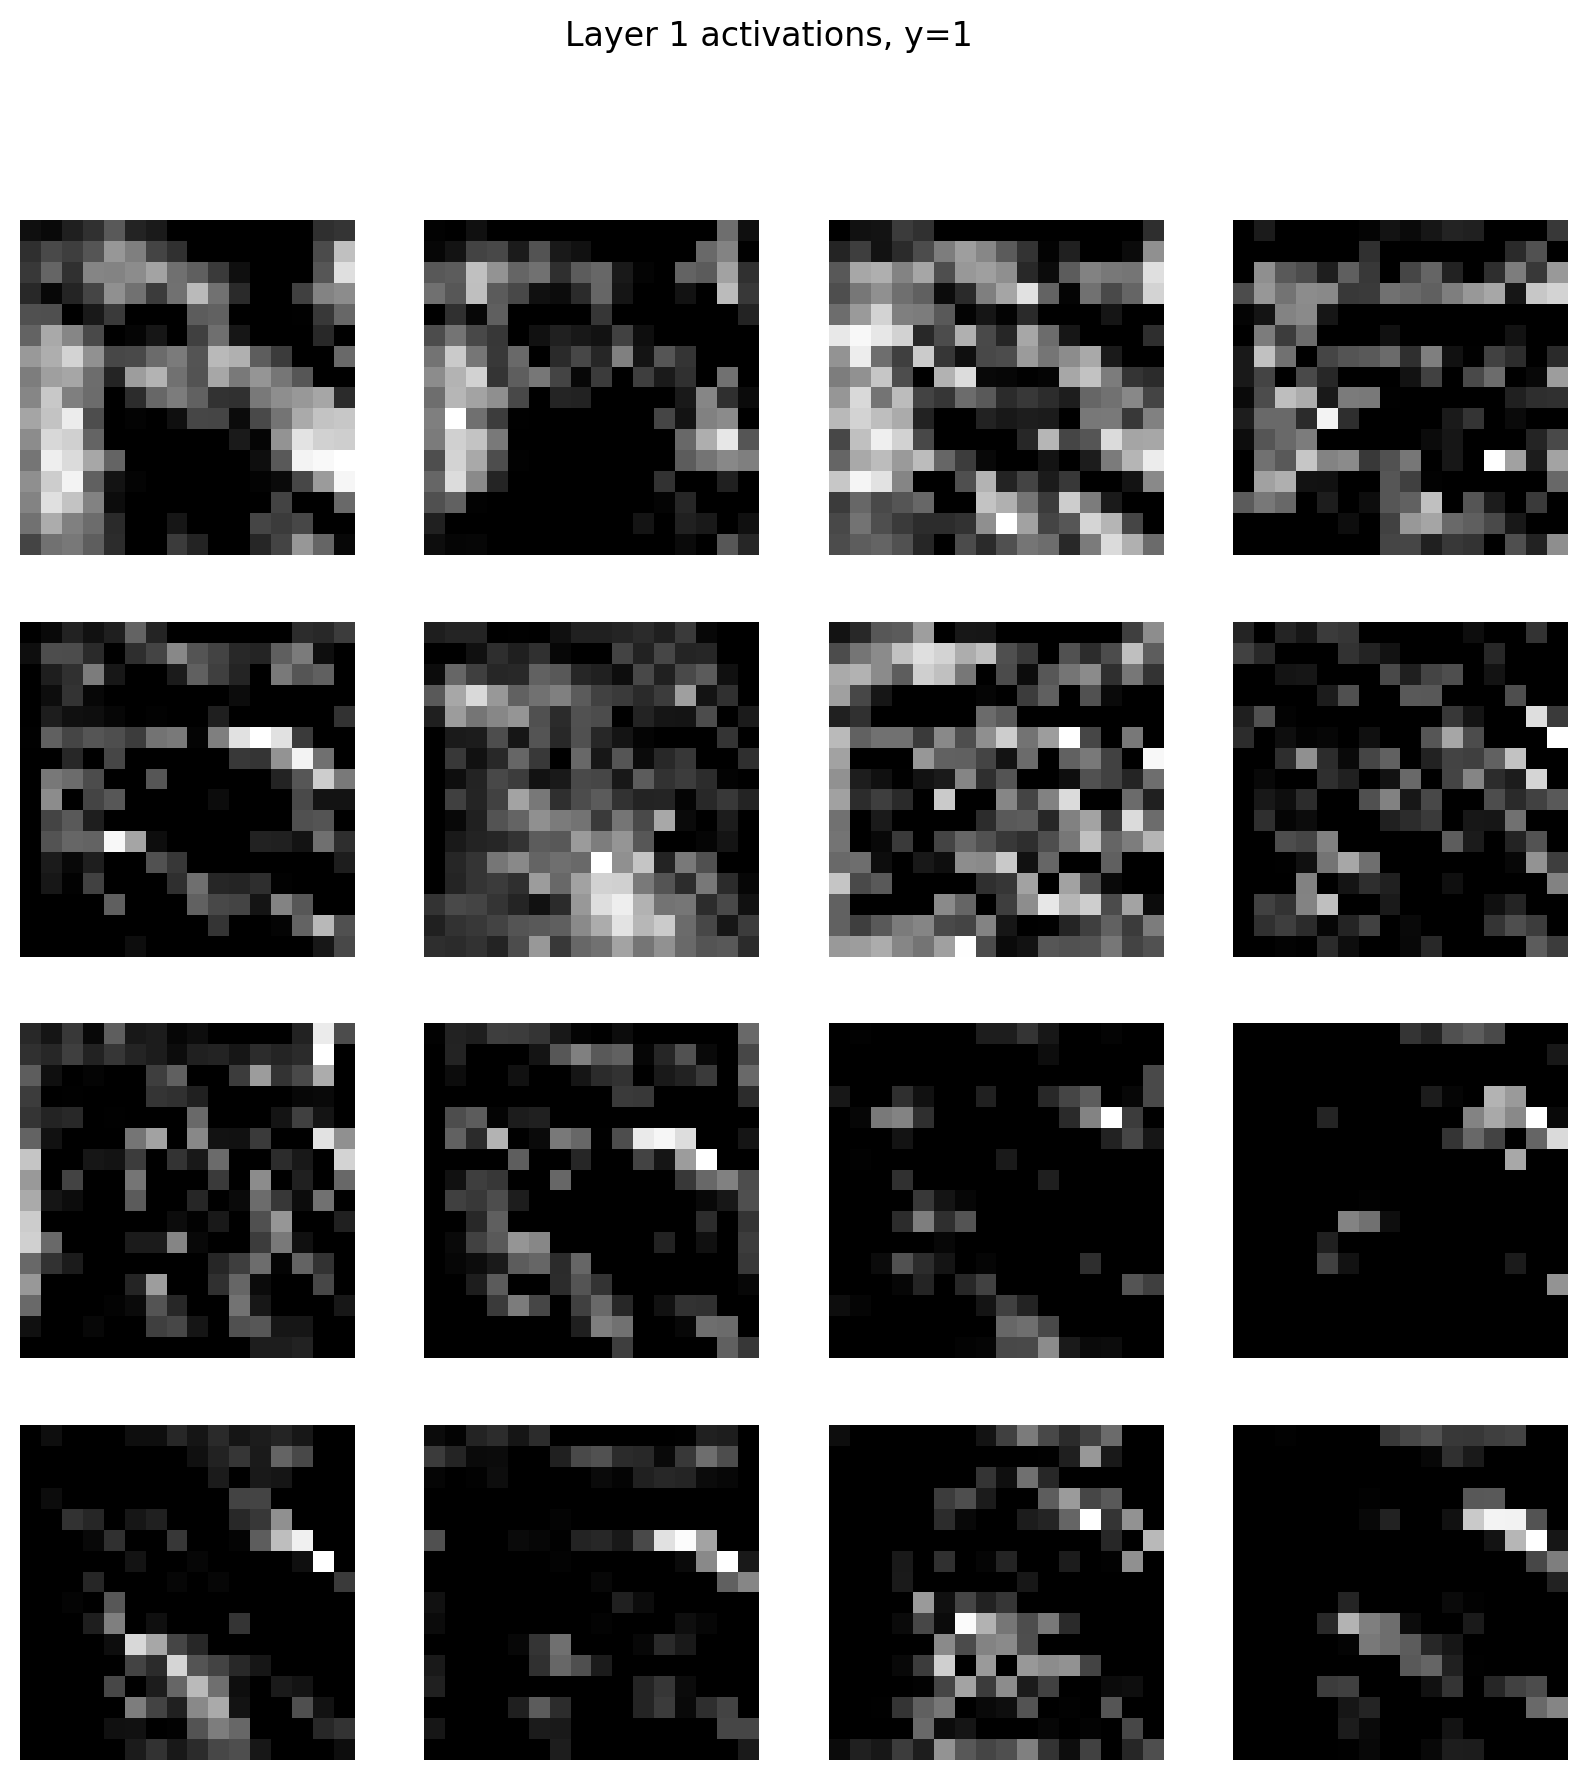
\includegraphics[scale=0.6]{CNN_viz1_1.png}
      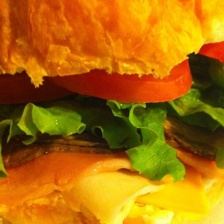
\includegraphics[scale=0.3]{00004.jpg}
      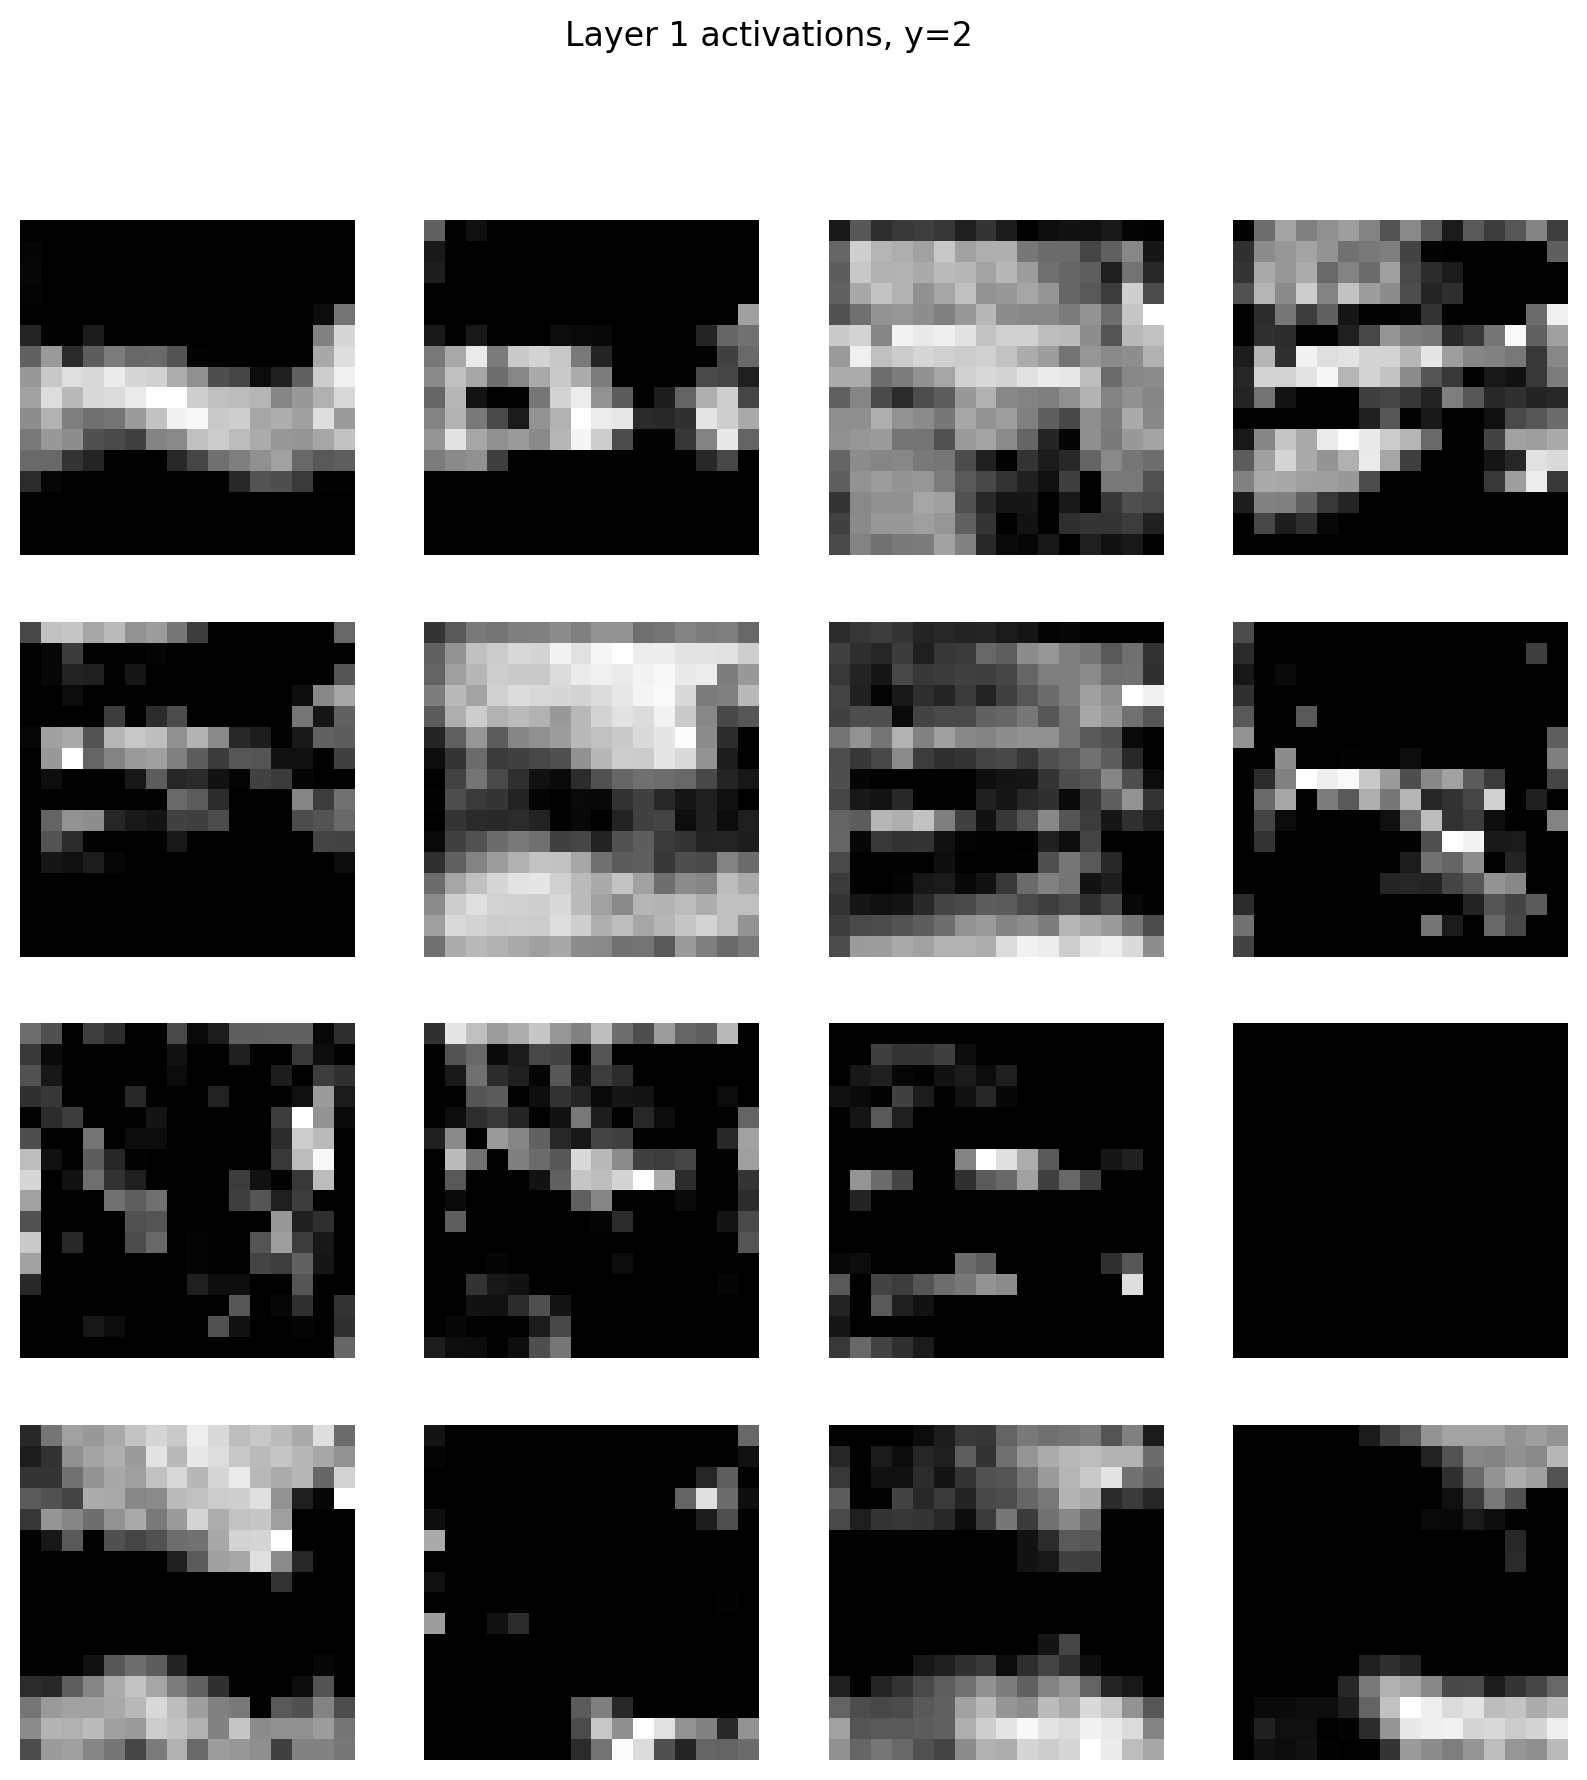
\includegraphics[scale=0.6]{CNN_viz1_2.png}
      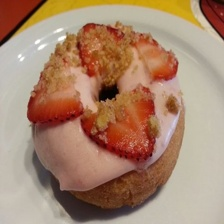
\includegraphics[scale=0.3]{00014.jpg}
      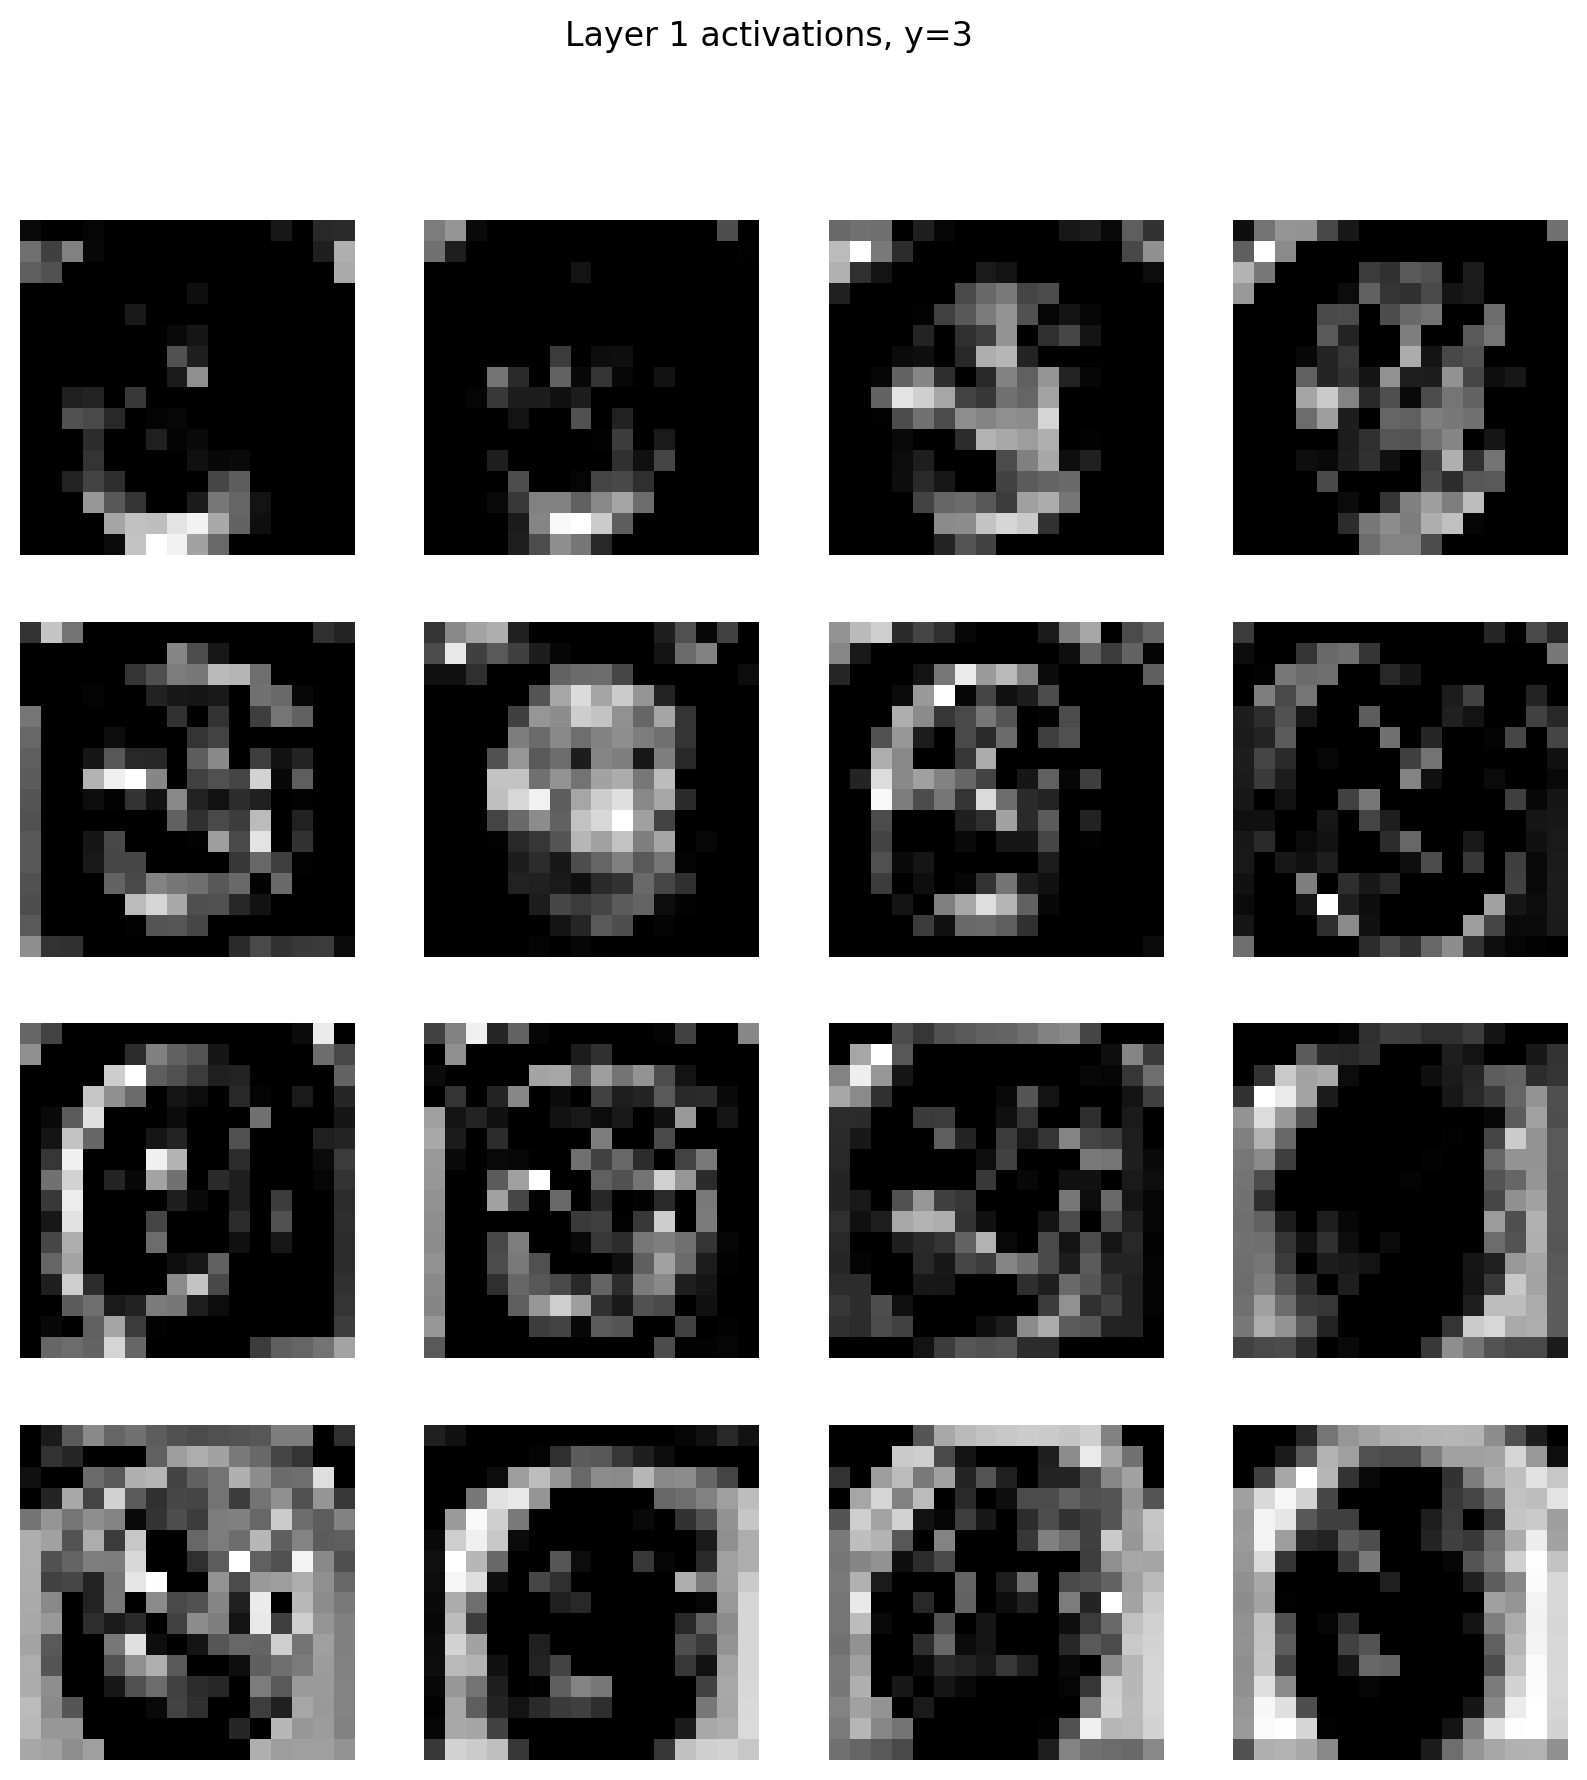
\includegraphics[scale=0.6]{CNN_viz1_3.png}
      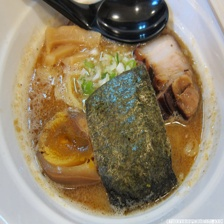
\includegraphics[scale=0.3]{00000.jpg}
      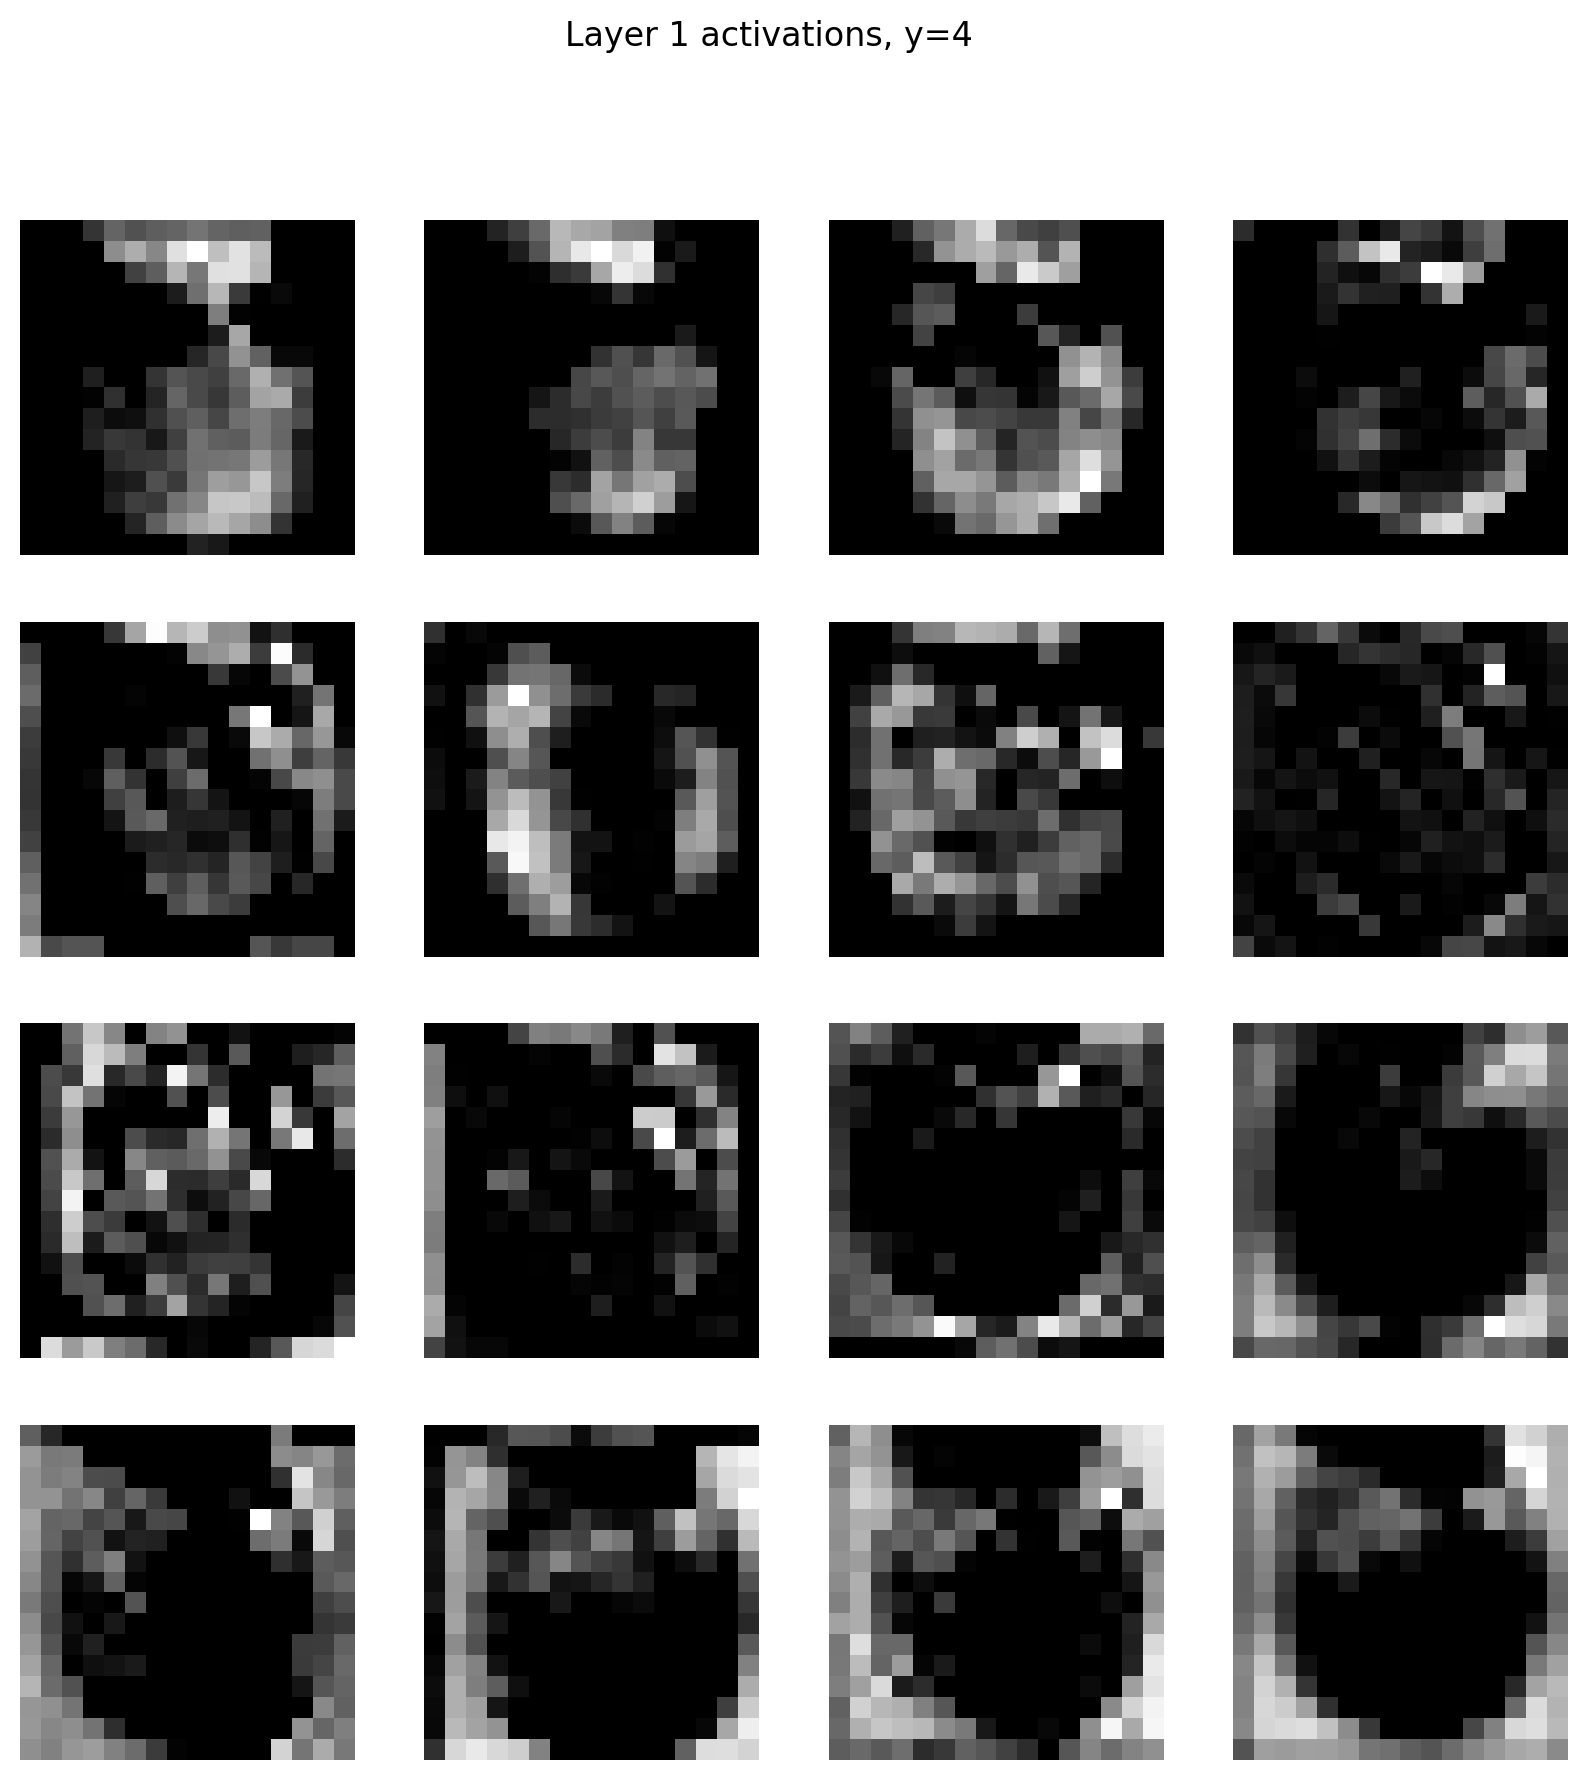
\includegraphics[scale=0.6]{CNN_viz1_4.png}
    \end{center}

    \begin{enumerate}[i.]
      \item For $y = 0, y = 3, y = 4$, the graphes all have plates, which is clearly captuared by last five filters, in which there are large bright circles. However, for $y = 1, y = 2$, the graphes do not have plates, so the last five filters of them do not have those features.

      \item Filter 1-7 might be looking for dark parts, while filter 11-16 might be looking for bright parts. Filter 8-10 might be looking for edges in different directions.
    \end{enumerate}



  \end{parts}
  \end{solution}

  \section{Classification by Autoencoder}%
  \label{sec:classification_by_autoencoder}

  \begin{solution}
    \begin{parts}
      \part 
      \begin{enumerate}[i.]
        \item Layers 2, 3 have weights corresponding to encoder, and layers 4, 5 have weights corresponds to decoder.
        \item  ~\\
        
        \begin{tabular}{c|ccccc}
        \hline
           & \multirow{2}{*}{Current} & \multirow{2}{*}{Alternative} & \multicolumn{3}{c}{How might the alternative choice affect...}\\
           \cline{4-6}
           & & & Training Spd & Struct Err & Est Err\\
           \hline
           Initialization& rdm normal& zero & $\downarrow$ & $\uparrow$ & $\downarrow$\\
           Activation& ELU& Sigmoid& $\downarrow$ & $\uparrow$ & $\downarrow$\\
           Depth& 4 & 6 & $\downarrow$ & $\downarrow$ & $\uparrow$\\
           Regularization& None & Dropout& $\downarrow$ & $\uparrow$ & $\downarrow$\\
           \hline
        \end{tabular}
        

        Initialization: If zero initialization is used instead of random normal initialization, then it is expected that the model will be much simpler, because many neurons will be learning the same information. As a result, the training speed will decrease dramatically because it is hard for the mordel to converge. Besides, as the model is simpler, the structual error will increase while the estimation error will decrease.

        Activation: ELU activation function converges only at the negative side while Sigmoid activation function converges at both sides. Therefore, it is expected that model with activation function of Sigmoid is simpler than that with activation function of ELU. As a result, the training speed will decrease, the structure error will increase while the estimation error will decrease.

        Depth: A model with largerr depth has more parameters, which indicates that the model has more complexity. Therefore, it will take more time to update, and the training speed will be slower. On the other hand, the structure error will decrease and the estimation error will increase.

        Regularization: The dropout layer actually makes the model a bit simpler, which leads to the result that the model may take longer time to converge and thus the training speed will decrease. Besides, the structure error will increase and the estimation error will decrease.
      \end{enumerate}

    \part
    \part
    \part The final training plot of validation MSE is shown below.
    \begin{center}
      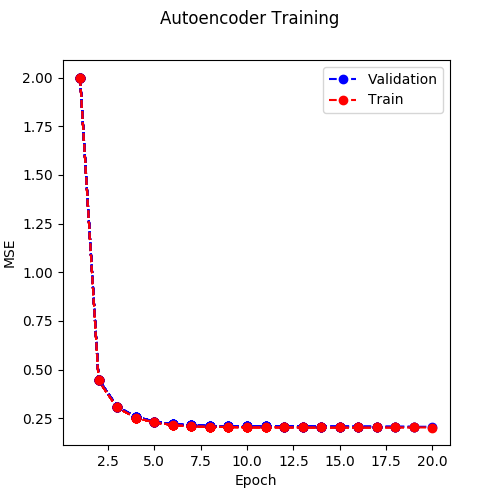
\includegraphics[scale=0.8]{eecs445-p2-3d.png}
    \end{center}

    MSE hardly changes after about epoch 10, which is considered as our stopping epoch number.

    \part

    \begin{enumerate}[i.]
      \item Since we have done normalization to make sure that the color space has mean 0 and variance 1, the baseline reconstruction MSE of the compression-decompression scheme that always returns the same reconstruction, a uniformly gray square is 1.

      \item ~\\
      \begin{tabular}{c|c}
        \hline
        Class& MSE\\
        \hline
        overall& 0.2217\\
        pasta& 0.2001\\
        salad& 0.2519\\
        snadwich& 0.2310\\
        cake& 0.2057\\
        soup& 0.2199\\
        \hline
      \end{tabular}

      \item ~\\
      \begin{center}
      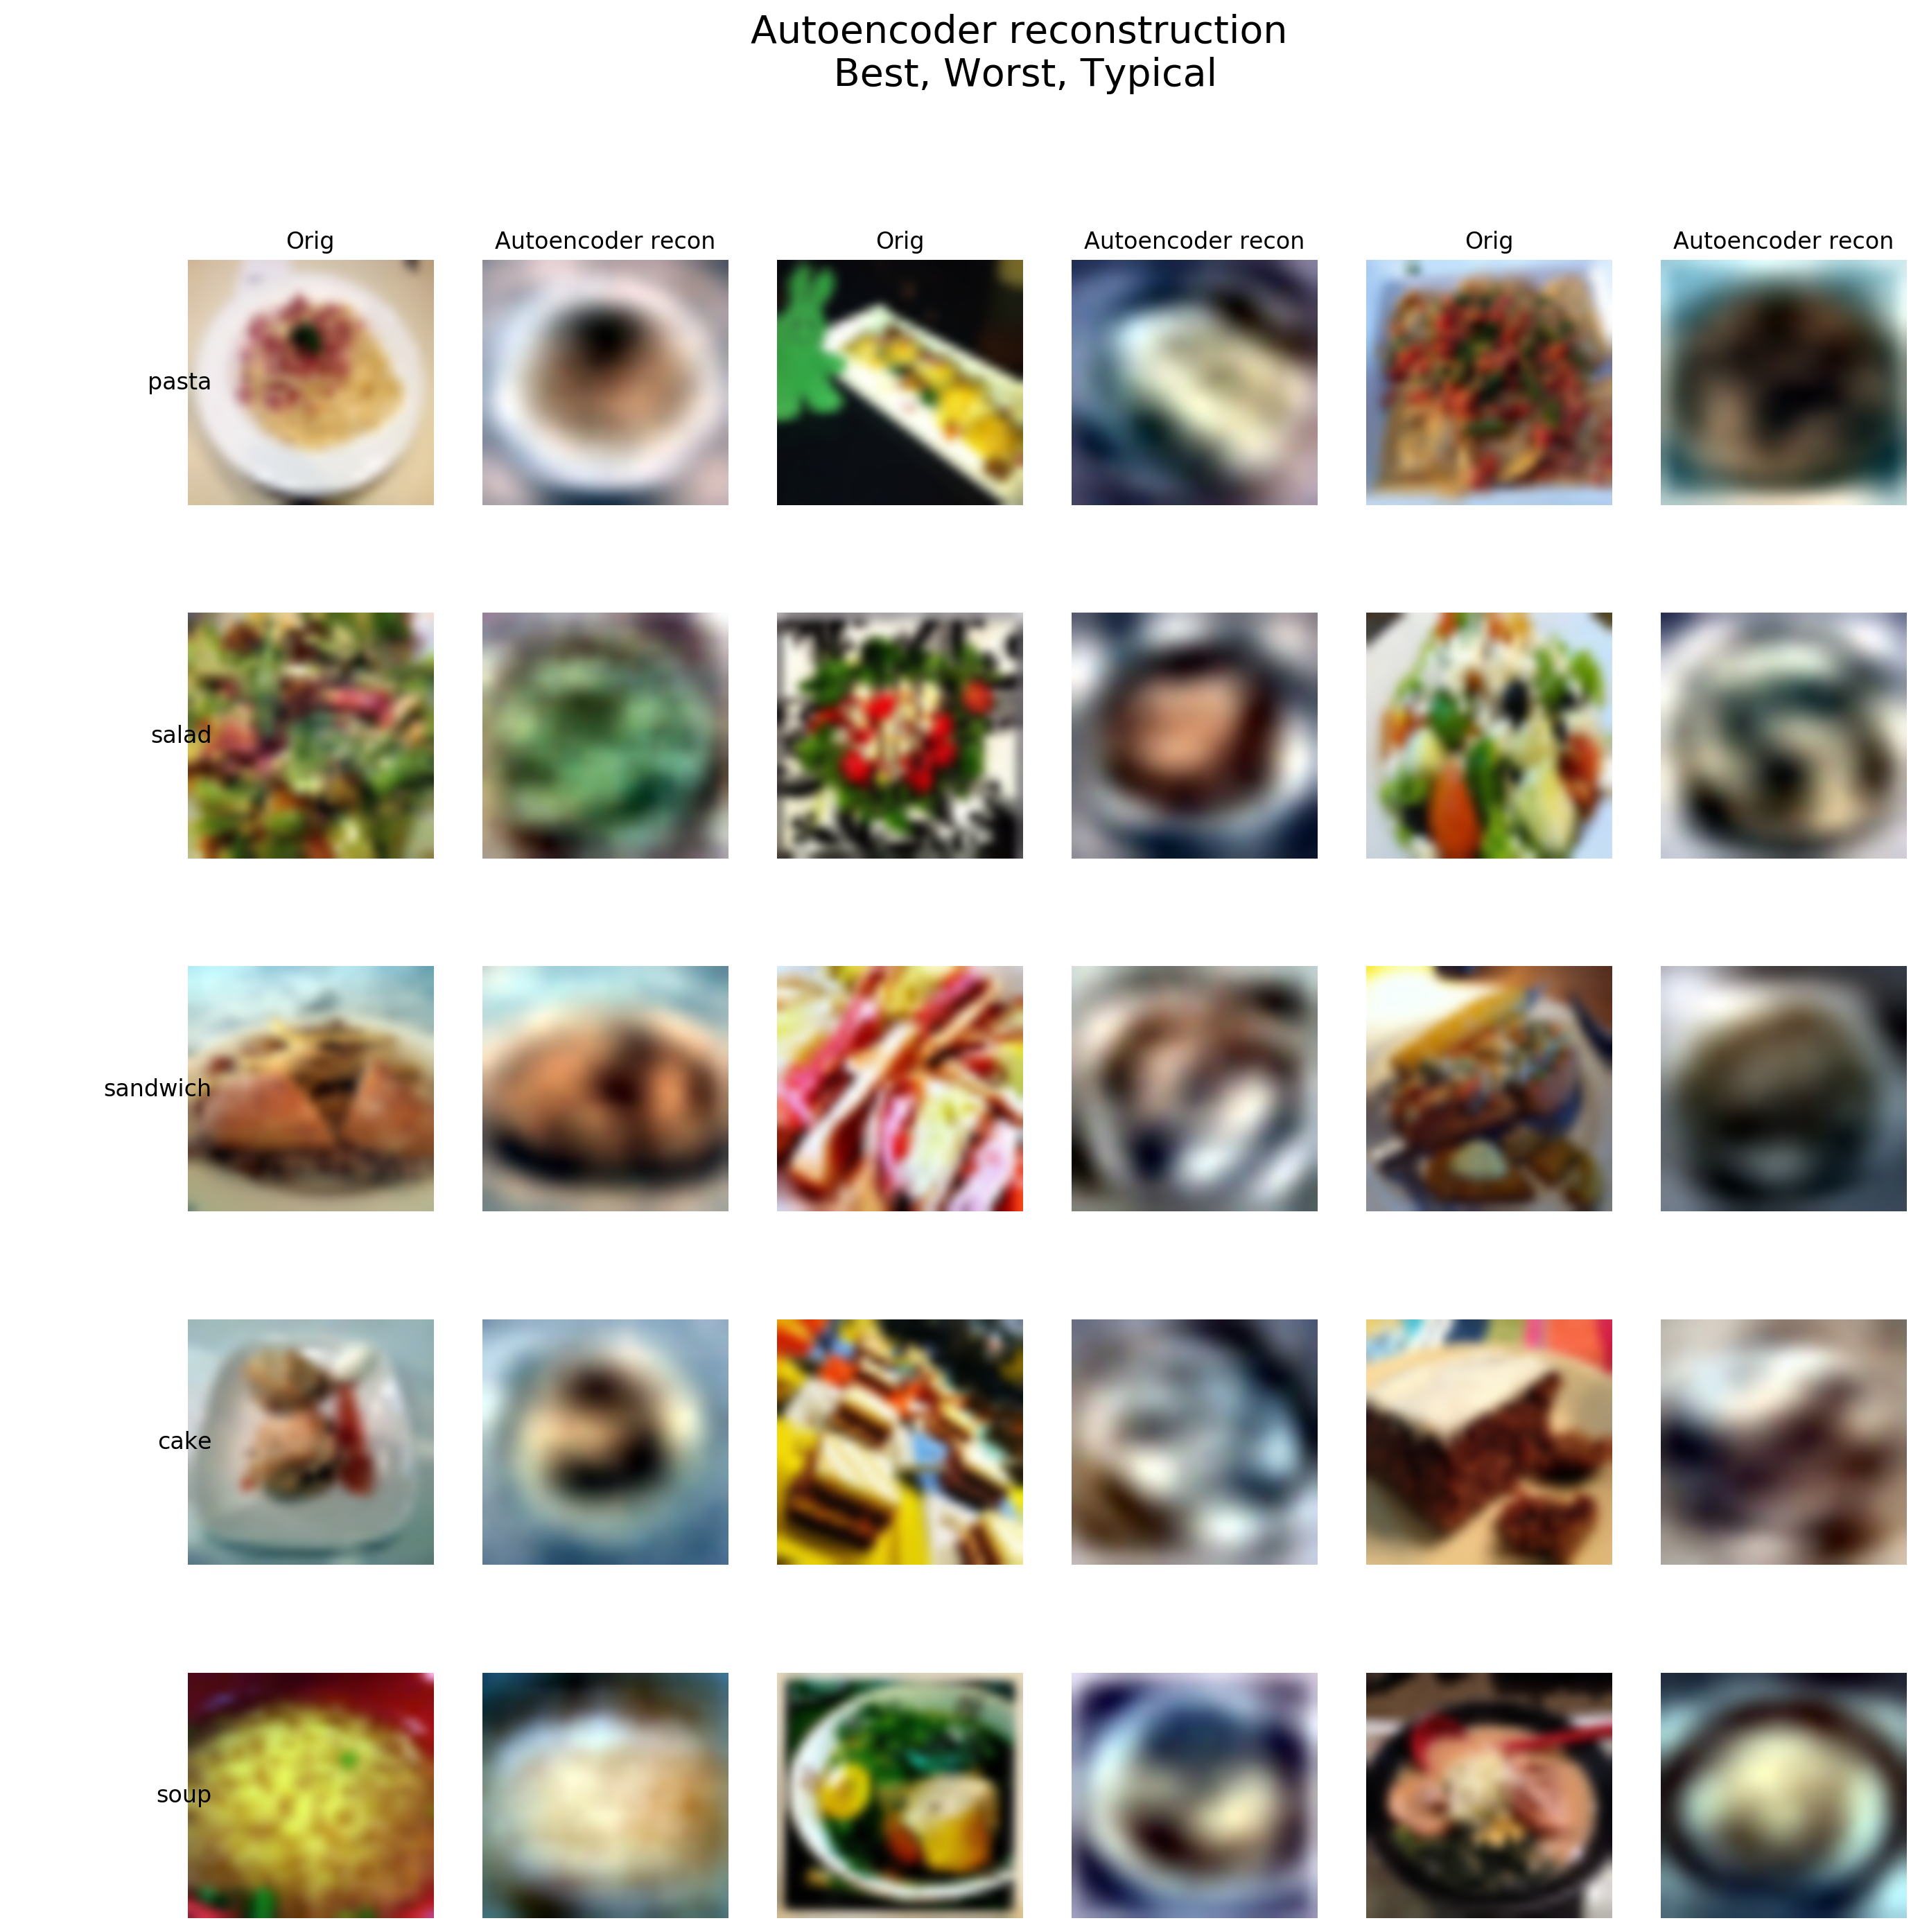
\includegraphics[scale=0.35]{ae_per_class_perf.png}
      \end{center}

      The encoder is best at reconstructing graphes where the food are in the middle and the picture is taken just in front of the food.
    \end{enumerate}
    
    \part ~\\
    \begin{center}
      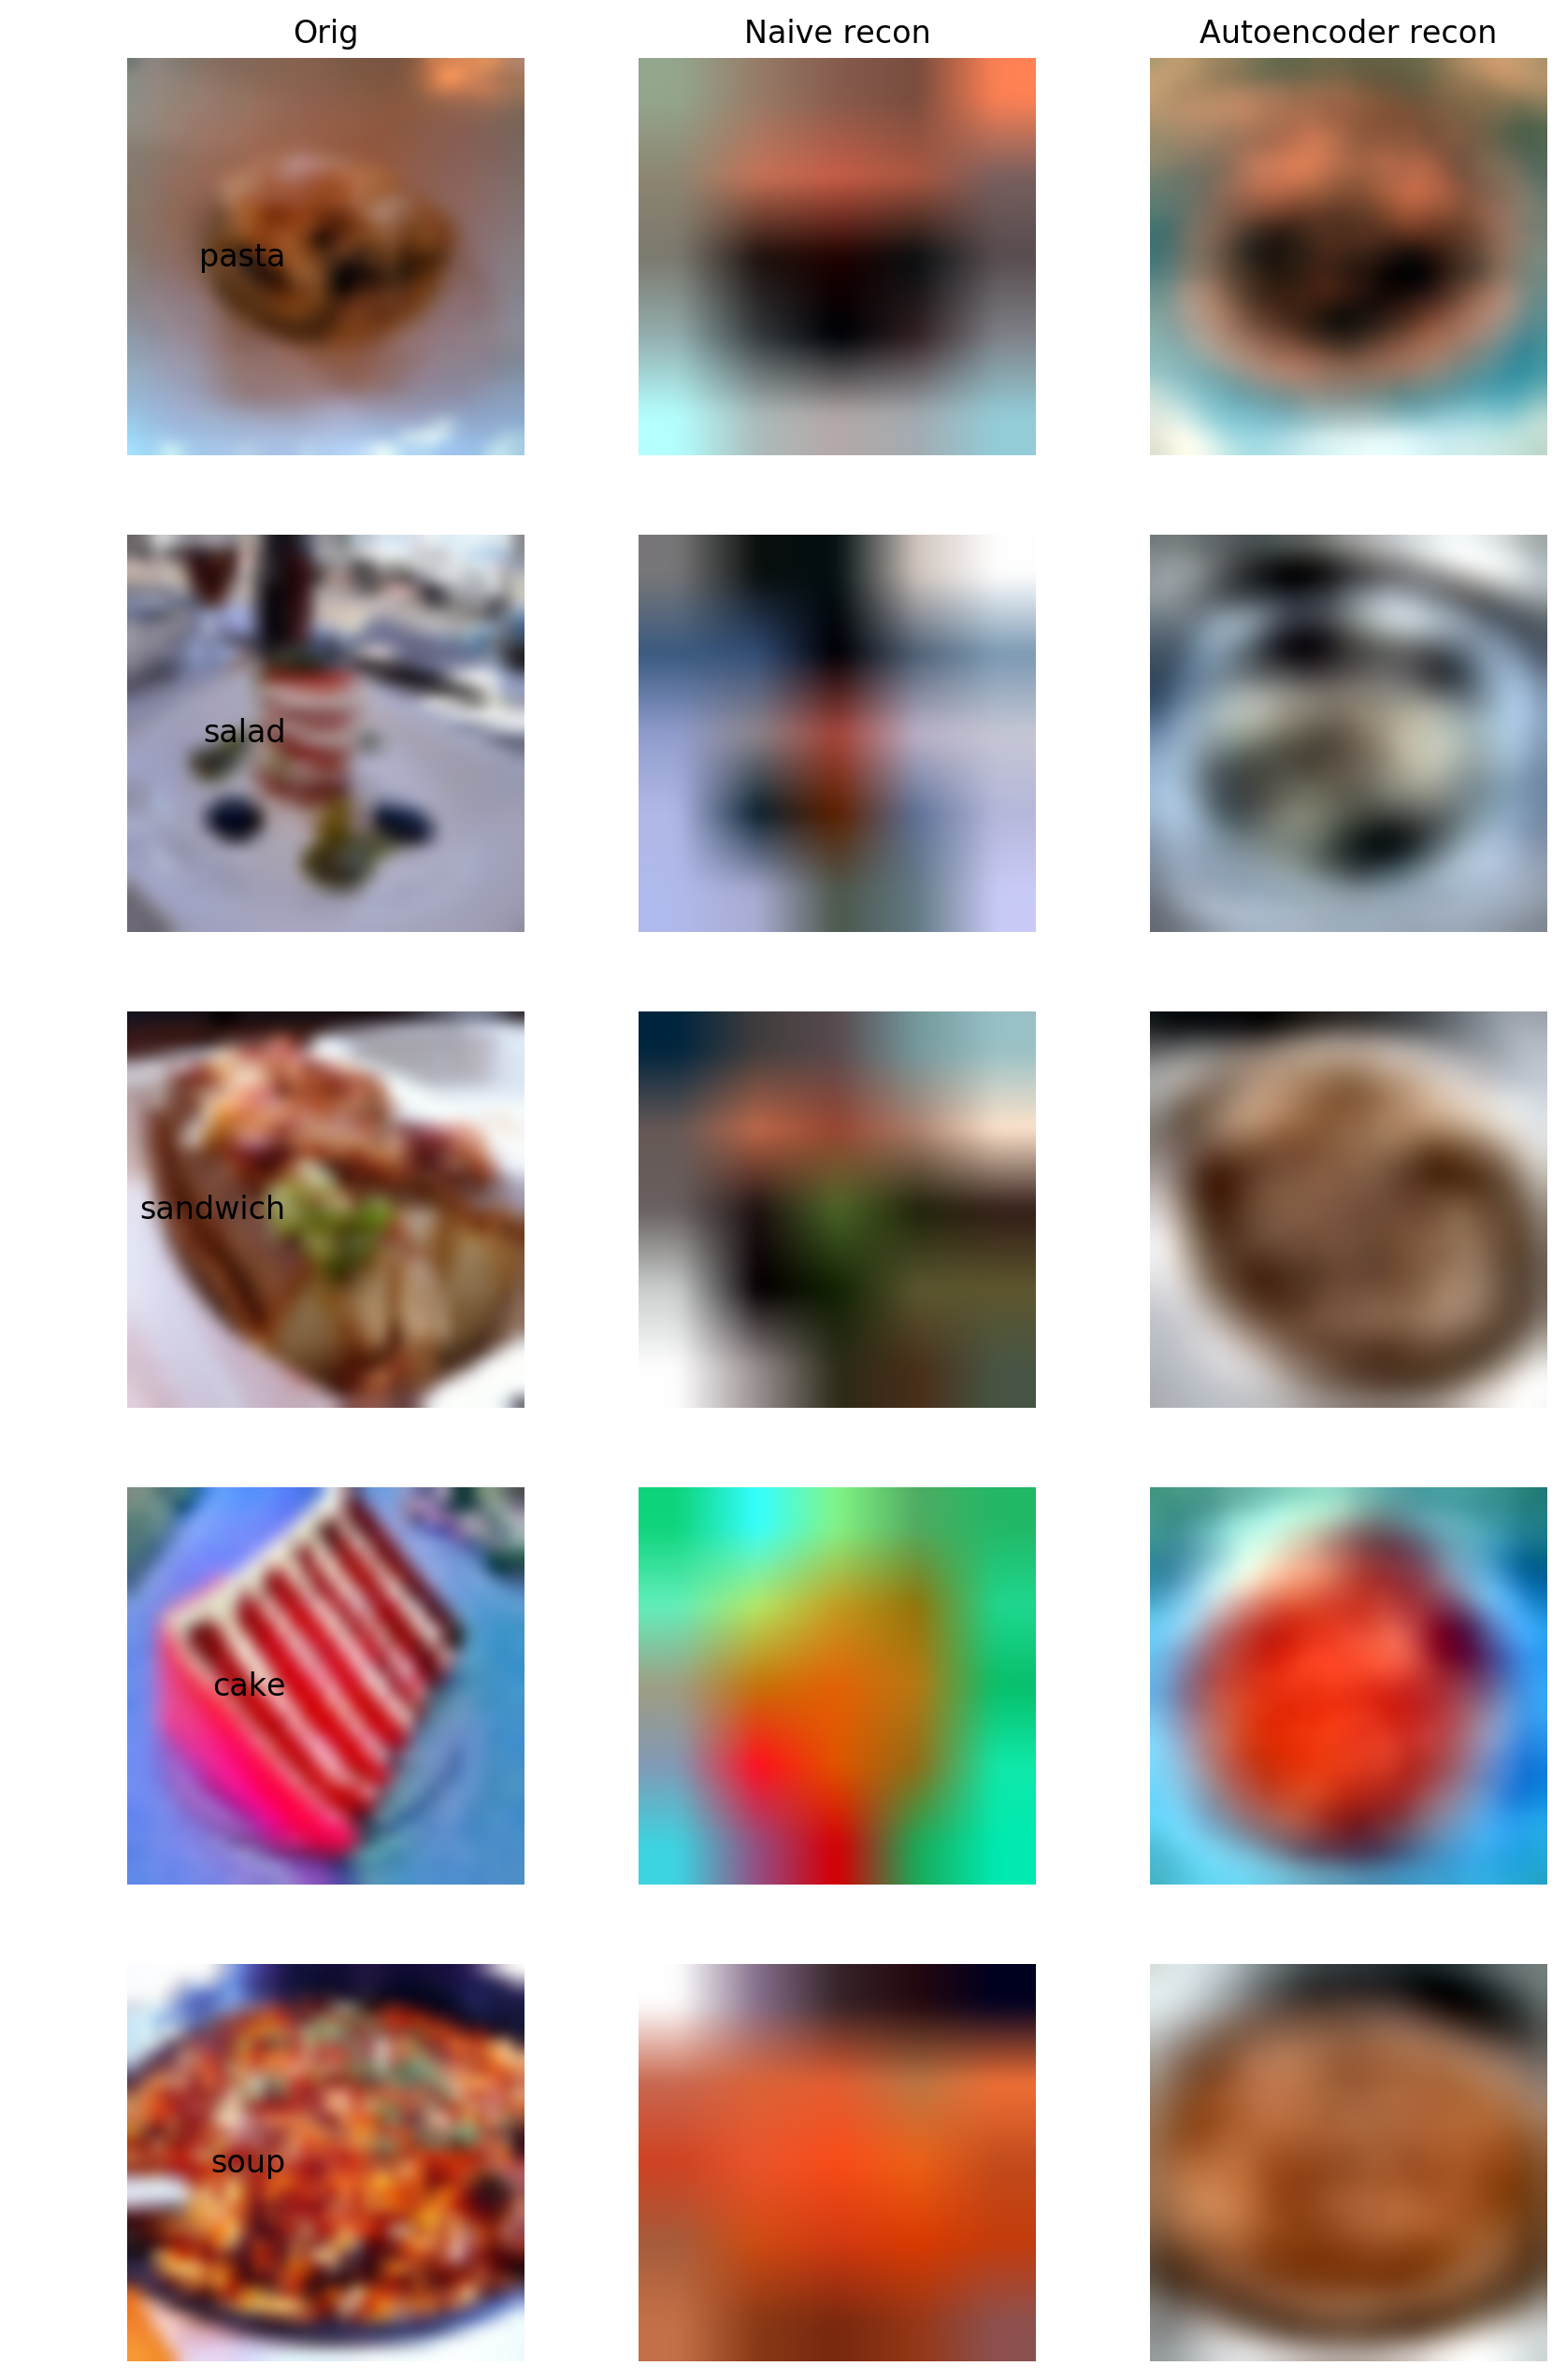
\includegraphics[scale=0.5]{ae_recon_comparison.png}
    \end{center}

    The autoencoder is much better than the naive reconstruction. 

    The naive reconstruction is similar with the resizing and standardization we have done in the preprocessing part. The images it produce are all blurry. On the other hand, the images produced by the autoencoder recognize some of the siginificant features of the original image, such as edges and shapes. Besides, it contains more information in terms of color. Taking the soup as an example. In the image reconstructed by the naive reconstruction, we can only see the blurry orange color. In contrast, in the image reconstructed by the autoencoder, we can roughly see what is in the soup. 

    \part ~\\
    \begin{tabular}{c|cc}
        \hline
        & CNN accuracy & Autoencoder classifier accuracy\\
        \hline
        y=0 pasta& 0.536 & 0.441 \\
        y=1 salad& 0.543 & 0.474 \\
        y=2 sandwich& 0.571& 0.350 \\
        y=3 cake& 0.621& 0.584 \\
        y=4 soup& 0.585& 0.351 \\
        \hline
    \end{tabular}

    The autoencoder classifier performs worse than the CNN, in terms of accuracy. However, the performance of autoencoder is still acceptable, not to mention that the training time cost by the autoencoder is less than that cost by CNN. The reason why the autoencoder classifier performs worse can be the fact that the original autoencoder (without the additional layers) actually aims to reconstruct the original image, instead of classifying. Therefore, it learns more features from the perspective of images, not from the perspective of classes. The difference might lead to the worse performance.

    It would be more suitable for an autoencoder classifier if the dataset we have is really large. In that case, it will be reasonable to use the autoencoder classifier which is faster and produce rather good results.




    \end{parts}
  \end{solution}



  \section{Classification by Autoencoder}%
  \label{sec:classification_by_autoencoder}
  \begin{solution}
    \begin{parts}
      
    \end{parts}
  \end{solution}

















\end{document}
